\chapter{连续}

\begin{figure}[ht]
  \centering
  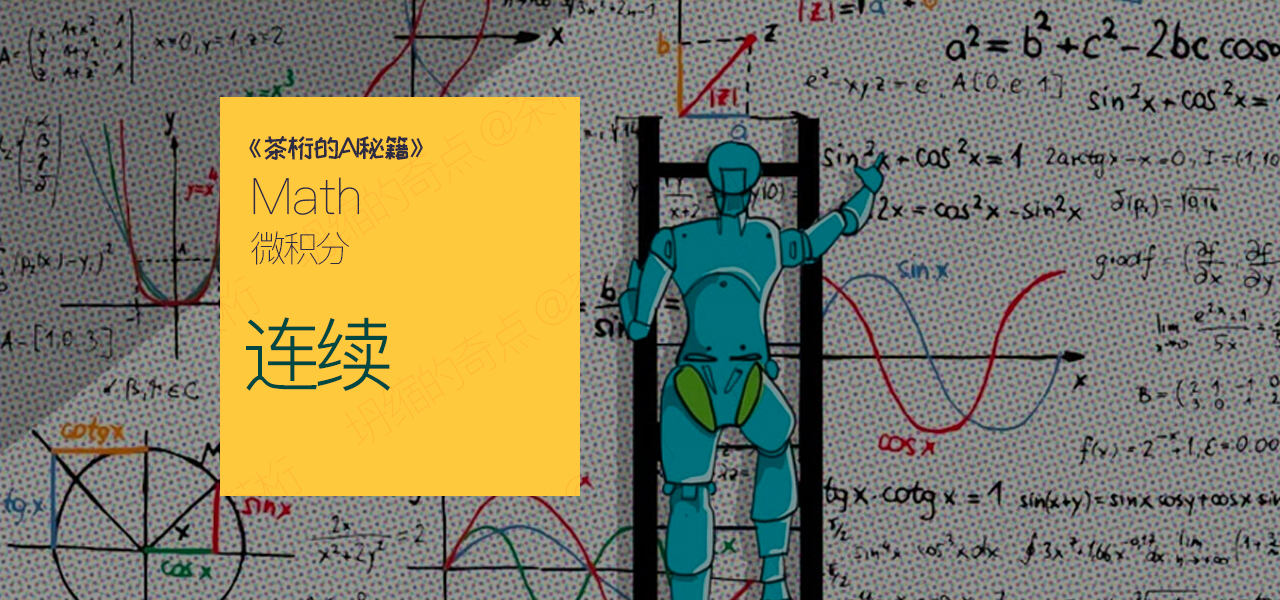
\includegraphics[width=1\textwidth]{asset/茶桁的AI秘籍_Math_8.png}
\end{figure}

\newpage

上一节课我们讲了极限, 很多小伙伴下来后跟我留言说有点懵. 不必太过在意, 慢慢的多看几遍去理解, 并且, 极限也并不是特别核心的问题, 暂时先放一放也可以. 

本节课, 我们要讲的内容是「连续」. 

\section{连续}

首先我们从直观上想一下, 在日常生活里面这个连续它给我们一些什么样的印象?可能会优先想到这么几点: 

\begin{itemize}
  \item 一个是不断裂. 
  \item 其次是不跳跃
  \item 处处相连
\end{itemize}

那咱们先来看第一点不断裂. 打比方说, 本来有这么一个函数图像好好的, 但是我们在它中间断了一个点, 就这么一个点就是一个老鼠屎坏了一锅粥. 连续就应该是不断裂的, 不能象图\ref{fig:img9_1}一样.

第二点是不跳跃. 如函数图\ref{fig:img9_2}, 这个函数本来在前面一段$x_0$这一点的函数值还在下面, 结果下一步就一下跃升到上面去了, 它有个跳跃. 这和我们日常生活中理解的连续也是不一样的. 

\begin{figure}[ht]
  \centering
  \begin{minipage}[h]{0.4\textwidth}
    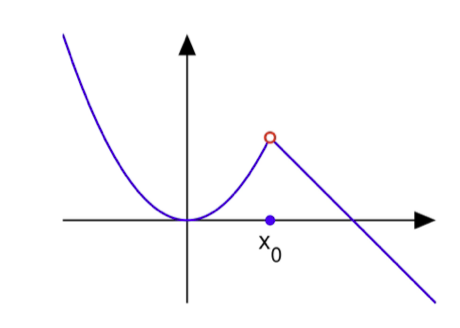
\includegraphics[width=\textwidth]{asset/aa29dda5-78fc-480a-b2ac-f1692445d496.png}
    \caption{断裂}
    \label{fig:img9_1}
  \end{minipage}%
  \hspace{2em}
  \begin{minipage}[h]{0.3\textwidth}
    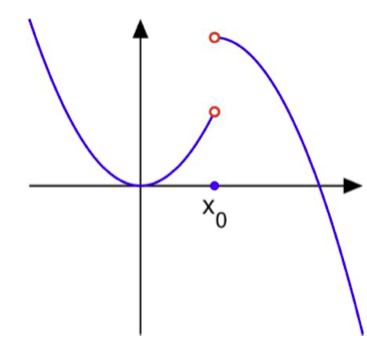
\includegraphics[width=\textwidth]{asset/63c70c64-4dda-41c6-94b5-9f88083516d0.png}
    \caption{跳跃}
    \label{fig:img9_2}
  \end{minipage}
\end{figure}

还有第三个: 处处相连. 其实只要不是上面这两种情况, 那基本上就是处处相连的. 如图\ref{fig:img9_3}, 就像我们当前这个图像所描述的一样, 任何一个地方都是连接在一起的, 就像一条锁链一样都是连接在一起的. 它并没有像上面两个函数图像一样出现断裂或者跳跃, 这个就是直观上面的. 

\begin{figure}[ht]
  \centering
  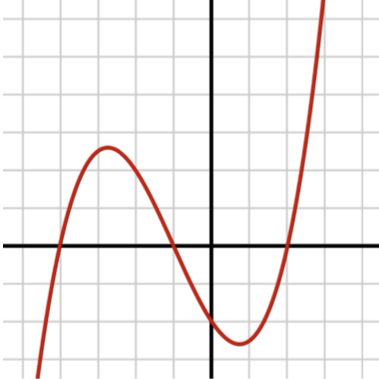
\includegraphics[width=0.3\textwidth]{asset/a5406854-3b3e-427c-b296-e56f004f1568.png}
  \caption{处处相连}
  \label{fig:img9_3}
\end{figure}

\paragraph{连续的正式定义如下}:

\begin{newquotation}
  设函数$f(x)$在点$x_0$的某个邻域内(例如:$(x_0 - 0.0001, x_0 + 0.0001)$)有定义, 如果有: \(\lim_{x \to x_0}f(x)=f(x_0)\), 则称函数f(x)在点$x_0$处连续, $x_0$称为函数$f(x)$的连续点. 
\end{newquotation}

定义中说: 函数$f(x)$在点$x_0$的某个邻域内, 邻域是什么意思呢?我们拿定义里的例如来说, $x_0$向左走了$0.0001$个单位, 然后$x_0$还向右走了$0.0001$个单位, 这个新的区间, 就称为$x_0$的邻域. 当然, 这个邻域的范围可以再小一点, 我们可以在这个单位前面再添加几个0. 如果函数$f(x)$在点$x_0$的某个邻域内有定义, 有定义就是这个蜡烛的光能照到这个手, 就叫做有定义. 要看懂我这个比喻需要前面的课上过是吧?也有可能有小伙伴没上过呢. 那好吧, 重新来说, 有定义就是可以映射. 

我们接着继续看, 如果有$\lim_{x \to x_0}f(x)=f(x_0)$这个式子, 那意思就是$f(x)$它在$x$趋近于$x_0$的时候, 极限的取值等于$f(x_0)$这个函数它在这一点的函数值, 我们就称它在点$x_0$处连续. 

稍微的来理解一下这个定义, 来看图\ref{fig:img9_4}: 

\begin{figure}[ht]
  \centering
  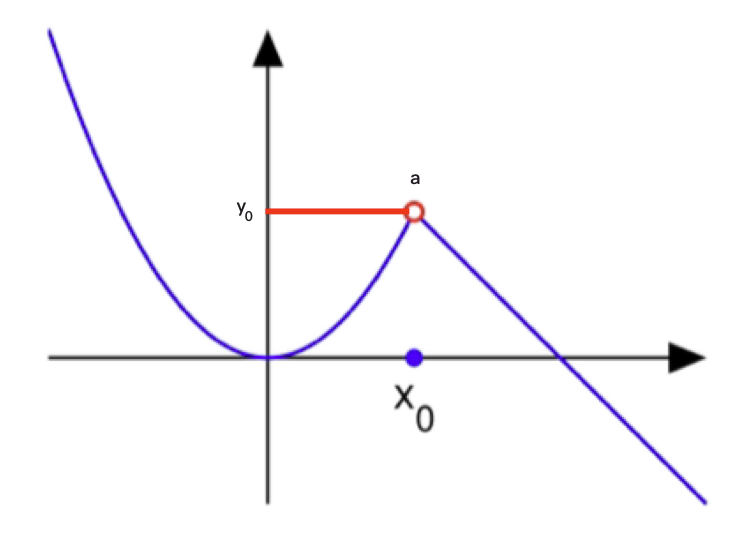
\includegraphics[width=0.4\textwidth]{asset/00036f9b-aad5-4c4e-b1a2-c7a287d93f1d.png}
  \caption{}
  \label{fig:img9_4}
\end{figure}

在$x_0$上方红圈$a$那一点的极限, 按照之前学的极限的概念来看, 在这里取值应该是对应的是趋近于a的值, 那么应该是趋近于$y_0$这么一个Y值, 但是函数在$x_0$的取值是等于0的, 也就是图中函数的$a$点值, 我们给它挖出来落在了X轴上, 这一点落在了X轴上面Y值就等于0. 所以函数在$a$这一点的函数值和它在这一节的极限不相等, 就出现了断裂. 

所以如果极限$\lim_{x \to x_0}f(x)$和$f(x_0)$这个函数值相等, 我们就说它在点$x_0$处是连续的, $x_0$也可以被称为函数$f(x)$的一个连续点. 

好吧, 我知道这个时候一定有些人又开始懵了. 如果学一个东西的时候, 能自己主动的去查去找解决办法是非常赞的. 但是也要给自己设立一个止损的时间. 有一个点如果自己一直想不通, 可能得换一种方法去解决他了. 比如说问一下其他人, 寻找一些其他可以引导你的方法. 网上很多课程所讲的角度和细节都不太一样, 有很多时候, 两篇文章的细节凑在一起的时候, 就忽然的开窍了. 或者也许, 以后我会忽然觉得那么讲好理解一点, 就再用其他方法讲一遍,忽然之间你就开窍了呢。

不管如何, 都要给自己设定一个止损时间, 如果你不给自己设一个时间, 会极大的损害学习的动力. 一开始的学习热情, 被一些一直攻不破的东西给消耗了, 这是一件得不偿失的事情. 

我们回过头来总结一下前面的内容, 可以说, 函数在连续点的极限就是连续点的函数值. 大家其实只要记住上面那一个图就行了. 明明在那一点上是连续的, 可是非要人为把a点的值挖出来放在x轴上, 也就是$x_0$这一点, 那肯定就变成不连续的了. 

接着, 我们来看一个证明: 

\begin{align*}
  \mbox{例子: } & \mbox{证明函数} f(x) = x^2, x \in R, \mbox{在 x=0处连续. } \\
  \mbox{解}: & \mbox{由题干易知}, f(0) = 0^2 = 0, \mbox{接下来验证}x = 0\mbox{处函数的极限值是否是}0: \\
  & \mbox{对任意} \varepsilon > 0, \mbox{取} \delta = \sqrt {\varepsilon},  \\
  & \mbox{则: } 0 < |x-0| < \delta , \\
  & \mbox{有: } |f(x) - 0 | = | x^2 - 0| < \delta ^2 = \varepsilon \\
  & \mbox{所以} f(x)\mbox{在 x= 0 处的极限为0} \\
  & \mbox{所以} f(x)\mbox{在x=0处连续}
\end{align*}

其实, 这个函数式, 我们在图上画一个函数图像就很清楚的看到结果. 不过肉眼看到的并不是百分百精确.

数学和物理有一点是不一样的. 物理提出一个假设, 然后去验证, 在已知范围内没有一个实验的结果是推翻他的, 或者说反驳他的, 那就可以承认这个理论是存在的. 但是数学不行, 只要没有证明全部的情况都是合理的, 都是符合这个假设的话, 都不能说它是一个真正的一个定理. 

所以, 数学和物理在这方面差别很大. 当然, 物理学虽然承认的一些定理其实也是有阶段性的. 像牛顿的万有引力定律, 或者说宏观物体的运动规律, 牛顿三定律在宏观、低速状态下其实是OK的. 但在微观或者说超高速的情况下其实又不存在了. 

所以物理理论自己也知道, 大概在哪些范围之内是存在的, 随时准备接受以后的这些实验来推翻或者说改进它. 

我们来看一下刚才这个证明的例子. 

首先判断一个函数是不是连续的怎么判断?我们看它的在这一点的函数值是什么, 在这一点函数值是$f(0) = 0$, 这个就没什么可说的. 接下来我们唯一需要做的就是$x=0$的时候函数的极限是否是0, 会不会跳到其他地方去, 就像图\ref{fig:img9_4}里面一样. 

在这里因为要考虑极限, 所以还是用上一节所说的极限的知识去做, 对于任意$\varepsilon > 0$,  然后取$\delta$等于$\sqrt{\varepsilon}$, 因为$\varepsilon$别人塞给你的你没法改, $\delta$可以自己随心所欲. 只要能证明出来下面那些就OK, 所以$\delta$其实是我们设计出来的. 然后$x-0$, 0这一点实际上就是$x_0$点, 它在这个范围之内的时候就有$f(x)$减去我们假设的这个极限, 然后就等于$|x^2 - 0|$, 也就是$x^2$的绝对值. 

当然了, $x^2$本身就是一个非负数, 绝对值也可以拿掉. 所以其实就是$x^2$. $x^2$根据式子是小于$\delta^2$的, 根据式子$\delta^2 = \varepsilon$,  那我们就恰好证明出来了, 函数值减去假设的极限, 确实小于任意的$\varepsilon$. 

这里的任意体现在什么地方?大家可以这样想,$\varepsilon$这里可以取0.01, 那这个时候$\delta$等于0.1, 这样带入进去一路算下来没有问题, $\varepsilon$再继续小, 比如说$10^{-10}$, 按照规则, 式子依然成立. 这个才是极限的魔力所在, 也是「任意」体现的地方. 

「任意」, 没什么数学基础的同学可能会想到什么?你刚才说的都是$\varepsilon$任意小, 那为啥不提这个$\varepsilon$特别大的情况? 其实, 特别大的情况没必要去考虑, 比如我告诉你一个数, 然后我让你猜大小, 你猜5, 我跟你说这个数比5还小, 那你会不会还往比5大的方向去猜?你会不会跟我说这数是不是10?不可能对吧?

所以虽然它是任意, 但其实我们去做这样的证明的时候, 关注的方向是他非常小的那么一刻. 因为只要非常小的时候都能满足这个式子, 那非常大的时候肯定是满足的. 所以虽然写的是「任意」这两个字, 但是大家要注意其实它真正关心的是$\varepsilon$非常小的情况. 

那我们就证明出来, $f(x)$在$x_0$处的极限就是0. 既然这个函数在这个点的极限是0, 函数值又是0, 那根据我们上面的结论, 这个函数就是在$x=0$处就连续了. 

OK, 极限、连续这两个比较痛苦的过程暂告一段落了. 因为大家以后如果去做AI算法工程师或者去做其他一些算法方面东西、AI模型方面的东西, 仍然有可能会涉及到这些数学方面的概念. 所以在这里大家也要有一个了解, 至少你要直观上面知道他描述了什么样的一个东西. 

如果不是如此, 大家甚至都可以选择略过这两节课. 当前我讲课主要是为了保证学科上的一个连续性. 
